\chapter{webs}
\label{sec:webs}
\lstset{style=68KStyle}

\begin{lstlisting}
web4: 
  dc.w 15 ; length of orientation table, number of channels in the web.
  dc.w 7  ; player's initial position on the web

  ; x/y pairs of all vertices in the web.
  dc.w 8,6,7,4,5,5,4,7    ;clover
  dc.w 6,8,4,9,5,11,7,12
  dc.w 8,10,9,12,11,11,12,9
  dc.w 10,8,12,7,11,5,9,4,8,6

  dc.w -1  ; Whether to join the last vertex with the first

  ;orientation table (angle of an object within a particular lane)
  dc.w -80,112,80,16,112,48,16,-48,48,-16,-48,-112,-16,-80,-112,80  
  dc.w $0,$70,$10,$60,$20,$50,$30,$40,$40,$30,$50,$20,$60,$10,$70,0

\end{lstlisting}

This is the routine that converts the web data structure into a list of vertices and lines between vertices
that will make up the web itself:

\begin{lstlisting}
extrude:
;
; extrude a web from a list of 16 pairs of XY coordinates addressed by (a1)
;
; a0 = vector ram space; a2.l = z depth to extrude to; d0-d7 as above

  move.l vadd,a0
  movem.l d0-d7/a0/a2,-(a7)    ;save so routine can return address
  clr connect
  move.l a2,-(a7)    ;save z depth
  bsr initvo    ;make header, do standard vector object init
  move.l a3,a4    ;save first vertex
  move.l (a7)+,d7    ;retrieve z-depth
  move d7,d0
  asr #1,d0
  move d0,web_z    ;Current Web z centering
  clr.l d0
  clr.l d1
  clr d5      ;to catch highest X point
  move (a1)+,d6            ; No of lines in the web.
  move d6,web_max          ; Keep it in web_max
  move (a1)+,web_firstseg  ; first position on web
  move.l a1,web_ptab       ;position table
  move.l a3,(a5)+          ;first vertex to lanes list
\end{lstlisting}

\begin{lstlisting}
  ; Read in the x/y pairs
xweb:
  ; Get the current x and y pair
  move (a1)+,d0
  move (a1)+,d1    ;get X and Y
  ext.l d0
  ext.l d1

  ; Check if this is the large X value so far
  cmp d5,d1       ; Compare x with the largest so far, stored in d5. 
  blt xweb2       ; If it's less, skip to xweb2 below.
  move d1,d5      ; It's bigger, so save it in d5.

xweb2:
  ; Store the x,y,z value for the near point in the web
  move.l d0,(a2)+ ; x value
  move.l d1,(a2)+ ; y value
  clr.l (a2)+     ; z value for near point (always 0)

  ; Store the x,y,z value for the far point in the web
  move.l d0,(a2)+ ; x value
  move.l d1,(a2)+ ; y value
  move.l d7,(a2)+ ; z value for far point (calculated by initvo).

  move d3,(a3)+    ;vertex ID to conn list
  tst d6
  beq lastpoint    ;special case for last point!

  ; Connect the vertices
  move d3,d4       ;copy vertex #
  addq #1,d4
  move d4,(a3)+    ;connect to n+1
  addq #1,d4
  move d4,(a3)+    ;connect to n+2
  move #0,(a3)+    ;end vertex 
  subq #1,d4       ;point to n+1
  move d4,(a3)+
  addq #2,d4       ;n+3
  move d4,(a3)+    ;connect
  move #0,(a3)+    ;delimit
  move.l a3,(a5)+  ;to v.conn list
  add #2,d3        ;move 2 vertices

  ; Get the next pair
  dbra d6,xweb
\end{lstlisting}

\begin{figure}[H]
    \centering
    \begin{adjustbox}{width=9cm,center}
      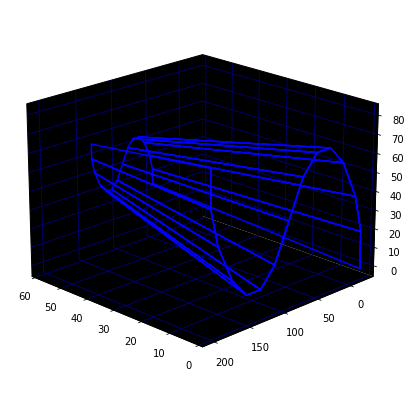
\includegraphics[width=12cm]{src/webs/sine_wave_no_title.png}%
    \end{adjustbox}
  \caption{Adding in our second triangle}
\end{figure}
